\chapter{Data description}

Our system is designed for data with a specific format and type so that the proposed algorithm can make use of them . In this chapter, two meeting transcripts and questions for these two meetings will be described. An analysis of this data, which also give the reasons to build our algorithm, is also presented. 

The questions used to test the system were created by the BET method. Thus, in order to have an overall view of this project as well as to understand features of the questions, we present a brief description of the BET method and the BET question in the first of the chapter.

\section{The BET method}
One method proposed originally by Flynn, M. and Wellner, P. \cite{flynn2003sgb} is the Browser Evaluation Test (BET). This method evaluates a meeting browser based on user performance rather than subjective judgment. According to the BET, the act of browsing a meeting recording is to an attempt to find a maximum number of \textit{observations of interest} in a minimum amount of time \cite{BET}, in which \textit{observations of interest} is defined as interesting to the meeting participants or to people who missed the meeting. Thus, the task of evaluating of a meeting browser is to collect a set of \textit{observations of interest} and then ask human subjects to verify these observations as binary-choice test questions in a fixed amount of time by using a meeting browser to access the meeting. A \textit{good} meeting browser will help human subjects find as many correct answers as possible in a shortest amount of time possible. Information on human subjects is described as answer precision (known as \textit{effectiveness}) and answer speed (known as \textit{efficiency}) which is used to evaluate the performance of the meeting browser. In detail, an \textit{observation of interest} is formed as a complementary pair of statements, one true and one false about a fact related to a meeting recording and human subjects are asked to determine which statement is true and which statement is false in the pair. The answer precision is calculated by dividing the number of correct answers over total answers. In terms of the answer speed, it is computed as the average time required to answer a question. Analyzing this information and comparing it among different meeting browsers provides scores for the performance of a meeting browser.

This is a time-consuming method that requires investment in collecting, preparing the observation and performing experiments with subjects. However, this observation collection is independent to browsers so that the observations collected can be extended to be used for the evaluation of other meeting browsers in the future. \cite{BET4TQB}.

The stages of the BET method is presented in the Figure \ref{fig1: BET stages}.

\begin{figure}[htbp]
\centering
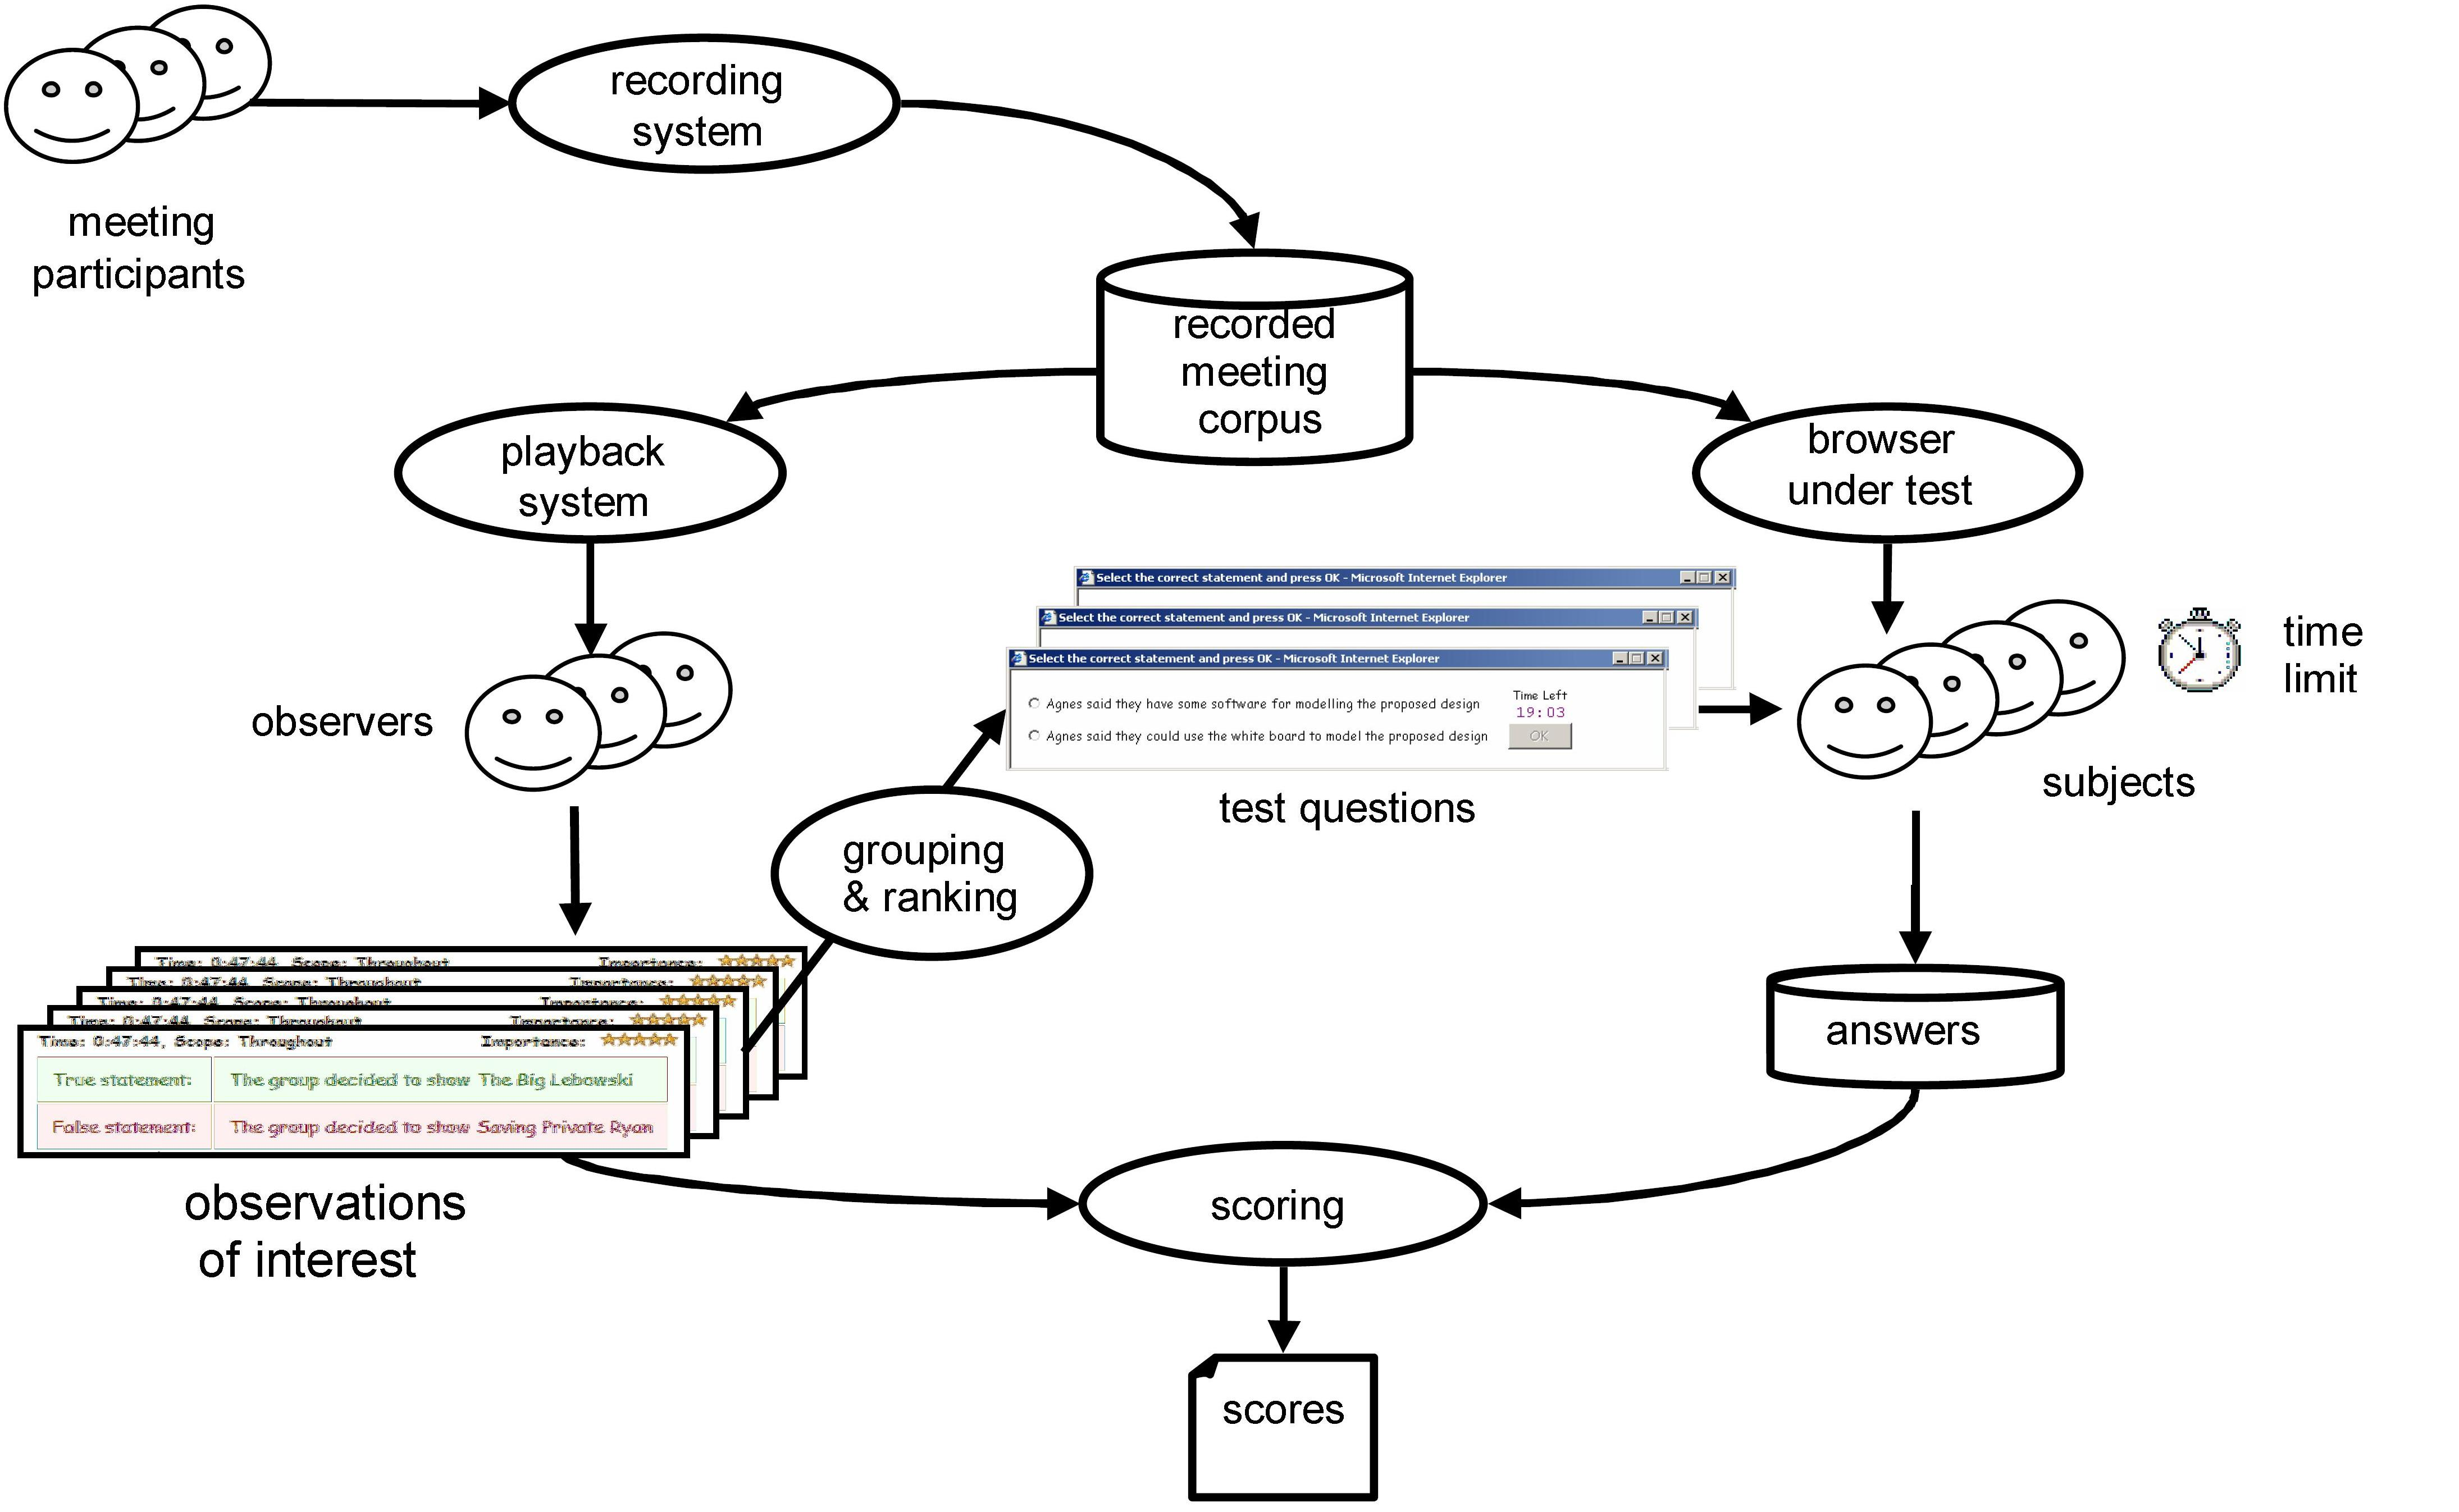
\includegraphics[scale = 0.15]{BET_stages.jpg}
\caption{Stages in the design and execution of a BET evaluation \cite{popescubelis:tbe}}\label{fig1: BET stages}
\end{figure}

\section{The BET Questions}
The pairs of statements used for the BET method, called the BET questions, are produced by a set of neutral observers, who independently watch selected meetings from corpus. These observers are native English speakers from the University of Sheffield. They are students, researchers and lecturers. The observers have unlimited time and access to the full recordings from such media sources as videos, audios, in parallel with paper printouts of the slides that participants worked on for the meeting. At first, an observer collects a list of observations that are true statements about facts or events that may interest meeting participants or people who missed the meeting. The collected statements should not be easy to guess without using the meeting information.  Then, for each true statement, a false counterpart statement is created so that a pair of complementary statements is generated. The observations should be simple and concisely stated.


An interface for observation collection is presented in the Figure \ref{fig2: create observations}. As seen in the Figure, there are three buttons "Nearby", "Around" and "Throughout" that indicate the position of information required to answer the question in the transcript. One observation is marked as \textit{Nearby} or \textit{Here} if it is pertinent to that particular moment; marked as \textit{Around} if it covers at least a minute of the meeting around the point the observer have selected; and marked as \textit{Throughout} if it broadly covers the whole meeting. However, in this system, the questions whose type is \textit{Throughout} are avoided because it is difficult to determine relevant passages which contain information required to  answer the questions using an automatic system. After that, the collected observations are examined by experts to reject repeated or inappropriate ones. 

\begin{figure}[htbp]
\centering
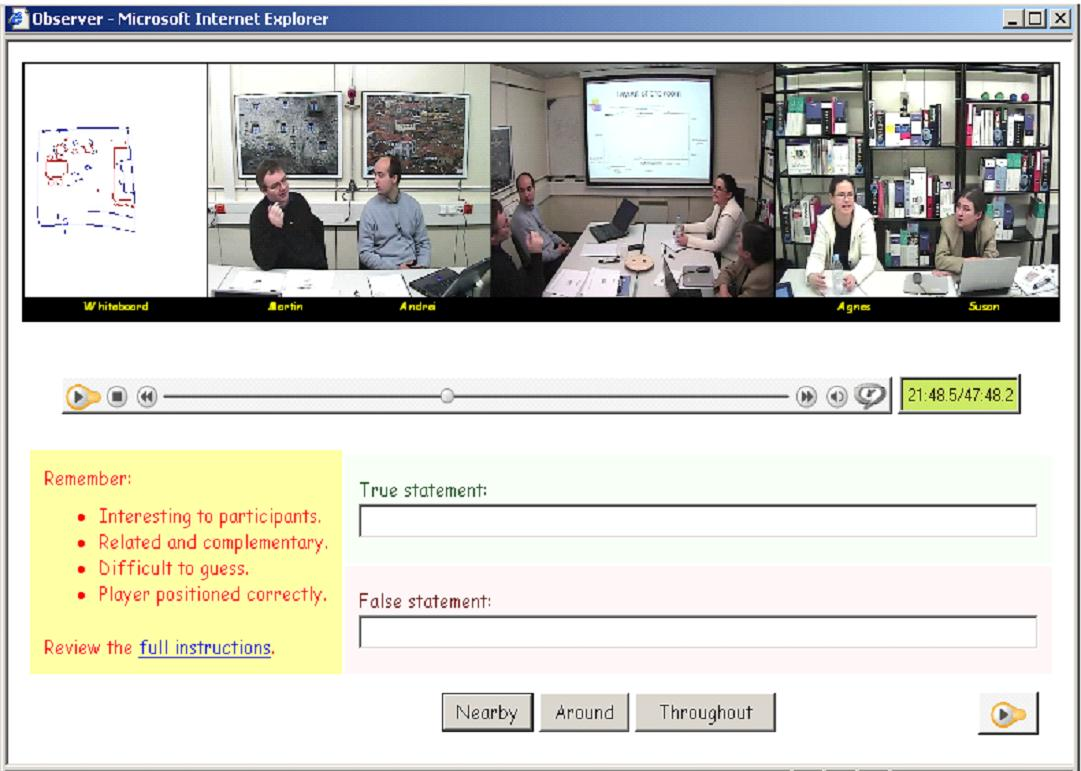
\includegraphics[scale = 0.5]{BET_interface.jpg}
\caption{Interface for observers}\label{fig2: create observations}
\end{figure}


\section{Data used to test the system}
\subsection*{Meeting transcripts}

Two meeting transcripts used to test the system were taken from the corpus built by the AMI project \cite{AMI_corpus}. Both of them are in English, involving four participants, native or non-native English speakers. The first meeting, IB4010, lasted 50 minutes in which managers of a movie club discussed how to select the movie for the next show. In the second meeting, IS1008c, a team discussed the design of a remote control for 26 minutes. There are two versions of the meeting transcripts, including manual and automatic ones. 

Unnecessary information from the original transcripts from AMI Corpus was eliminated such as time of utterances and notations of episodes. Consequently, the most important information left in the two manual meeting transcripts is speaker name and utterances that are showed in the Tables \ref{transcript_IB4010} and \ref{transcript_IS1008c}.

In a conversational document such as a meeting transcript, information about speakers plays an important role in answering the questions that verify a statement with respect to the speaker of one/some utterances. That is why in the proposed algorithm, in order to calculate passage scoring, we pay more attention to the name of speakers in both questions and transcript. For instance, score for a matched word as speaker name is the highest compared to other matched words.


%\begin{table}[htbp]
%\footnotesize
%\caption{Description of meeting transcript}
%\begin{center}
%\begin{tabular}{|lp{5cm}|lp{5cm}|}
%\hline
%\multicolumn{ 2}{|c|}{\textbf{Movie club meeting (IB4010)}} & \multicolumn{ 2}{c|}{\textbf{Remote control design meeting (IS1008c)}} \\ \hline
%\multicolumn{1}{|c}{\textbf{Speaker}} & \multicolumn{1}{c|}{\textbf{Utterances}} & \multicolumn{1}{c}{\textbf{Speaker}} & \multicolumn{1}{c|}{\textbf{Utterances}} \\ \hline
%Andrei  & Hi everyone.  & Sridhar  & so if you find out from the technology background, okay, so that would be good.  \\ 
%Denis  & So I don't know if you all received the the a- agenda for this meeting.  Do you - no?  & Christine  & Sounds good.  \\ 
%Mirek  & No, I haven't.  & Agnes  & Why was the plastic eliminated as a possible material?  \\ 
%Denis  & Here it is.  & Christine  & Because um it gets brittle, .. cracks -  \\ 
%Mirek  & Thank you.  & Christine  & We want - we expect these um uh these remote controls to be around for several hundred years.  Good expression.  \\ 
%Agnes  & I haven't.  & Ed  & Good expression.  \\ 
%Denis  & So um um the goal for today are um - We have two goals. Uh - First is to decide a movie for uh the next projection for our movie club.  & Christine  & I don't know, speak for yourself, I'm planning to be around for a while.  \\ 
%Mirek  & Mm-hmm.  & Agnes  & Although I think - \$ I think with wood though you'd run into the same types of problems, wouldn't you? I mean, it chips, it- if you drop it, uh it's - I'm not sure \$  \\ 
%Andrei  & Mm-hmm.  & Sridhar  & So so you're not convinced* about the the wood, yes.  \\ 
%... & ... & ... & ... \\ \hline
%\end{tabular}
%\end{center}
%\label{Meeting transcript}
%\end{table}


\begin{table}[htbp]
\caption{Meeting transcript IB4010}
\begin{tabular}{|lp{12cm}|lp{0cm}|}
\hline
Andrei & Hi everyone. \\
Denis & So I don't know if you all received the the a- agenda for this meet-
ing. Do you � no? \\ 
Mirek & No, I haven't. \\ 
Denis & Here it is. \\
Mirek & Thank you. \\
Agnes & I haven't. \\ 
Denis & So um um the goal for today are um - We have two goals. Uh - First is to decide a movie for uh the next projection for our movie club. \\ 
Mirek & Mm-hmm. \\ 
Andrei & Mm-hmm. \\ 
... & ... \\  \hline
\end{tabular}
\label{transcript_IB4010}
\end{table}


\begin{table}[htbp]
\caption{Meeting transcript IS1008c}
\begin{tabular}{|lp{12cm}|lp{0cm}|}
\hline
Agnes & Why was the plastic eliminated as a possible material? \\
Christine & Because um it gets brittle, .. Cracks �  We want - we expect these um uh these remote controls to be around for several hundred years. 
Good expression. \\ 
Ed & Good expression. \\ 
Christine & I don't know, speak for yourself, I'm planning to be around for a while. \\ 
Agnes & Although I think - \$ I think with wood though you'd run into the same types of problems, wouldn't you? I mean, it chips, it- if you drop it, uh it's - I'm not Sure \$ \\ 
Sridhar & So so you're not convinced* about the the wood, yes. \\  
... & ... \\  \hline
\end{tabular}
\label{transcript_IS1008c}
\end{table}



\subsection*{Questions}

The BET Questions have been mentioned above. However, some information of the questions used in this system are eliminated from full versions of original BET questions, which consists of miscellaneous information such as observation time, mediate time, important level, scope, etc. \cite{BET}.  The system needs only the true and the false statement in each question, which are considered as input data to distinguish one from another. Examples of some pairs are in the Tables \ref{questions_IB4010} and \ref{questions_IS1008c}.


For the two meetings IB4010 and IS1008c, 222 and 217 raw observations were collected by 9 and 6 observers respectively. After being filtered and corrected, the results are only 116 and 50 final pairs of true/false statement.

\begin{table}[htbp]
\caption{The BET questions IB4010}
\begin{tabular}{|lp{12cm}|lp{0cm}|}
\hline
True & Mirek had not received the agenda for the meeting \\
False & Andrei had not received the agenda for the meeting \\ \hline
True & None has seen the Shawshank redemption \\ 
False & Only two have seen the Shawshank redemption \\ \hline
True & Denis informed the team that the first objective was to choose a film and the second was
to discuss an advertising poster \\ 
False & Denis informed the team that the first objective was to choose a film and the second was to discuss a date for the film to be shown \\ \hline
... & ... \\ \hline
\end{tabular}
\label{questions_IB4010}
\end{table}

\begin{table}[htbp]
\caption{The BET questions IS1008c}
\begin{tabular}{|lp{12cm}|lp{0cm}|}
\hline
True & One of the features under consideration is speech recognition. \\ 
False & One of the features under consideration is fingerprint identification. \\ \hline
True & The product is expected to last over several hundred years. \\ 
False & The product is expected to last more than 5 but less than 15 years. \\ \hline
True & Christine eliminated plastic as too brittle over time. \\ 
False & Christine eliminated plastic as it would flex and damage the chips.  \\ \hline
... & ... \\ \hline
\end{tabular}
\label{questions_IS1008c}
\end{table}


%\begin{table}[htbp]
%\footnotesize
%\caption{Description of the BET Questions}
%\begin{center}
%\begin{tabular}{|l|p{7cm}|p{7cm}|}
%\hline
% & \textbf{Movie club meeting (IB4010)} & \textbf{Remote control design meeting (IS1008c)} \\ \hline
%True & Mirek had not received the agenda for the meeting & One of the features under consideration is speech recognition. \\ 
%False & Andrei had not received the agenda for the meeting & One of the features under consideration is fingerprint identification. \\ \hline
%True & None has seen the Shawshank redemption & The product is expected to last over several hundred years. \\ 
%False & Only two have seen the Shawshank redemption & The product is expected to last more than 5 but less than 15 years. \\ \hline
%True & Denis informed the team that the first objective was to choose a film and the second was to discuss an advertising poster & Christine eliminated plastic as too brittle over time. \\ 
%False & Denis informed the team that the first objective was to choose a film and the second was to discuss a date for the film to be shown & Christine eliminated plastic as it would flex and damage the chips \\ \hline
%... & ... & ... \\ \hline
%\end{tabular}
%\end{center}
%\label{The BET Questions}
%\end{table}

The fact that the questions considered as statements is one main feature that makes this system different than other question answering systems, which normally consists of different questions like "How", "Why", "When", etc. For this reason, it is not necessary to apply an existing complex algorithm, which was widely used to deal with various type of questions in other question answering systems. Therefore, our proposed algorithm is designed to try to fit the type of the BET questions. In this case, a typical question ask to verify information spoken by a speaker, for instance "Mirek asks who has seen Schindlers List". In this case, they have a speaker name at the beginning of the sentence. According to our statistics, there are over 55\% of such questions (28/50 such questions for IS1008c and 87/116 such questions for IB4010). This is an important remark that score of one matched word spoken by speaker whose name is mentioned in both the transcript and the question should be higher than other matched words.

Another feature of the questions is the similarity of two statements in a pair. In most pairs, two statements are different from each other by only one or two words. Therefore, at the Passage Retrieval stage of the proposed algorithm the probability that the two found corresponding passages coincide is very high. In this case, the true and the false statement can be distinguished by the similarity between each candidate statement with the corresponding passage. In other words, passage score for each statement is compared to determine the true statement/the false statement.

%Remain questions seem to be straightforward.